%
% Modified by Sameer Vijay
% Last Change: Wed Jul 27 2005 13:00 CEST
%
%%%%%%%%%%%%%%%%%%%%%%%%%%%%%%%%%%%%%%%%%%%%%%%%%%%%%%%%%%%%%%%%%%%%%%%%
%
% Sample Notre Dame Thesis/Dissertation
% Using Donald Peterson's ndthesis classfile
%
% Written by Jeff Squyres and Don Peterson
%
% Provided by the Information Technology Committee of
%   the Graduate Student Union
%   http://www.gsu.nd.edu/
%
% Nothing in this document is serious except the format.  :-)
%
% If you have any suggestions, comments, questions, please send e-mail
% to: ndthesis@gsu.nd.edu
%
%%%%%%%%%%%%%%%%%%%%%%%%%%%%%%%%%%%%%%%%%%%%%%%%%%%%%%%%%%%%%%%%%%%%%%%%

%
% Chapter 4
%

\chapter{MUON VETO DEVELOPMENT}
\label{chap:muVeto}
Explain some cosmic ray basics - only the stuff relevant to our detector (1 muon per square foot per second and MIP -> landau energy distribution).
Discuss materials available for veto and basic design decision of WLS

\section{Light Collection with WLS}
Describe light collection with WLS
Explain why we loop the WLS and collect light from both ends
Discuss the light limitations of light guides (Liouville) and ways to increase light collection with WLS (more!)
Describe fragility of WLS, how some efforts make custom plastic clamps to make it robust, how this doesn't work for you so you made a break and attached a cable.  Discuss signal loss.

\section{Paddle Design}
Schematics
Tolerances
Making sure the transmit cable lines up wih the paddle WLS fibers!  Dowels.  Tolerance doesn't actually need to be that good
connecting cable with PMT
cable design - hosing for protection

\begin{figure}[ht]
\centering
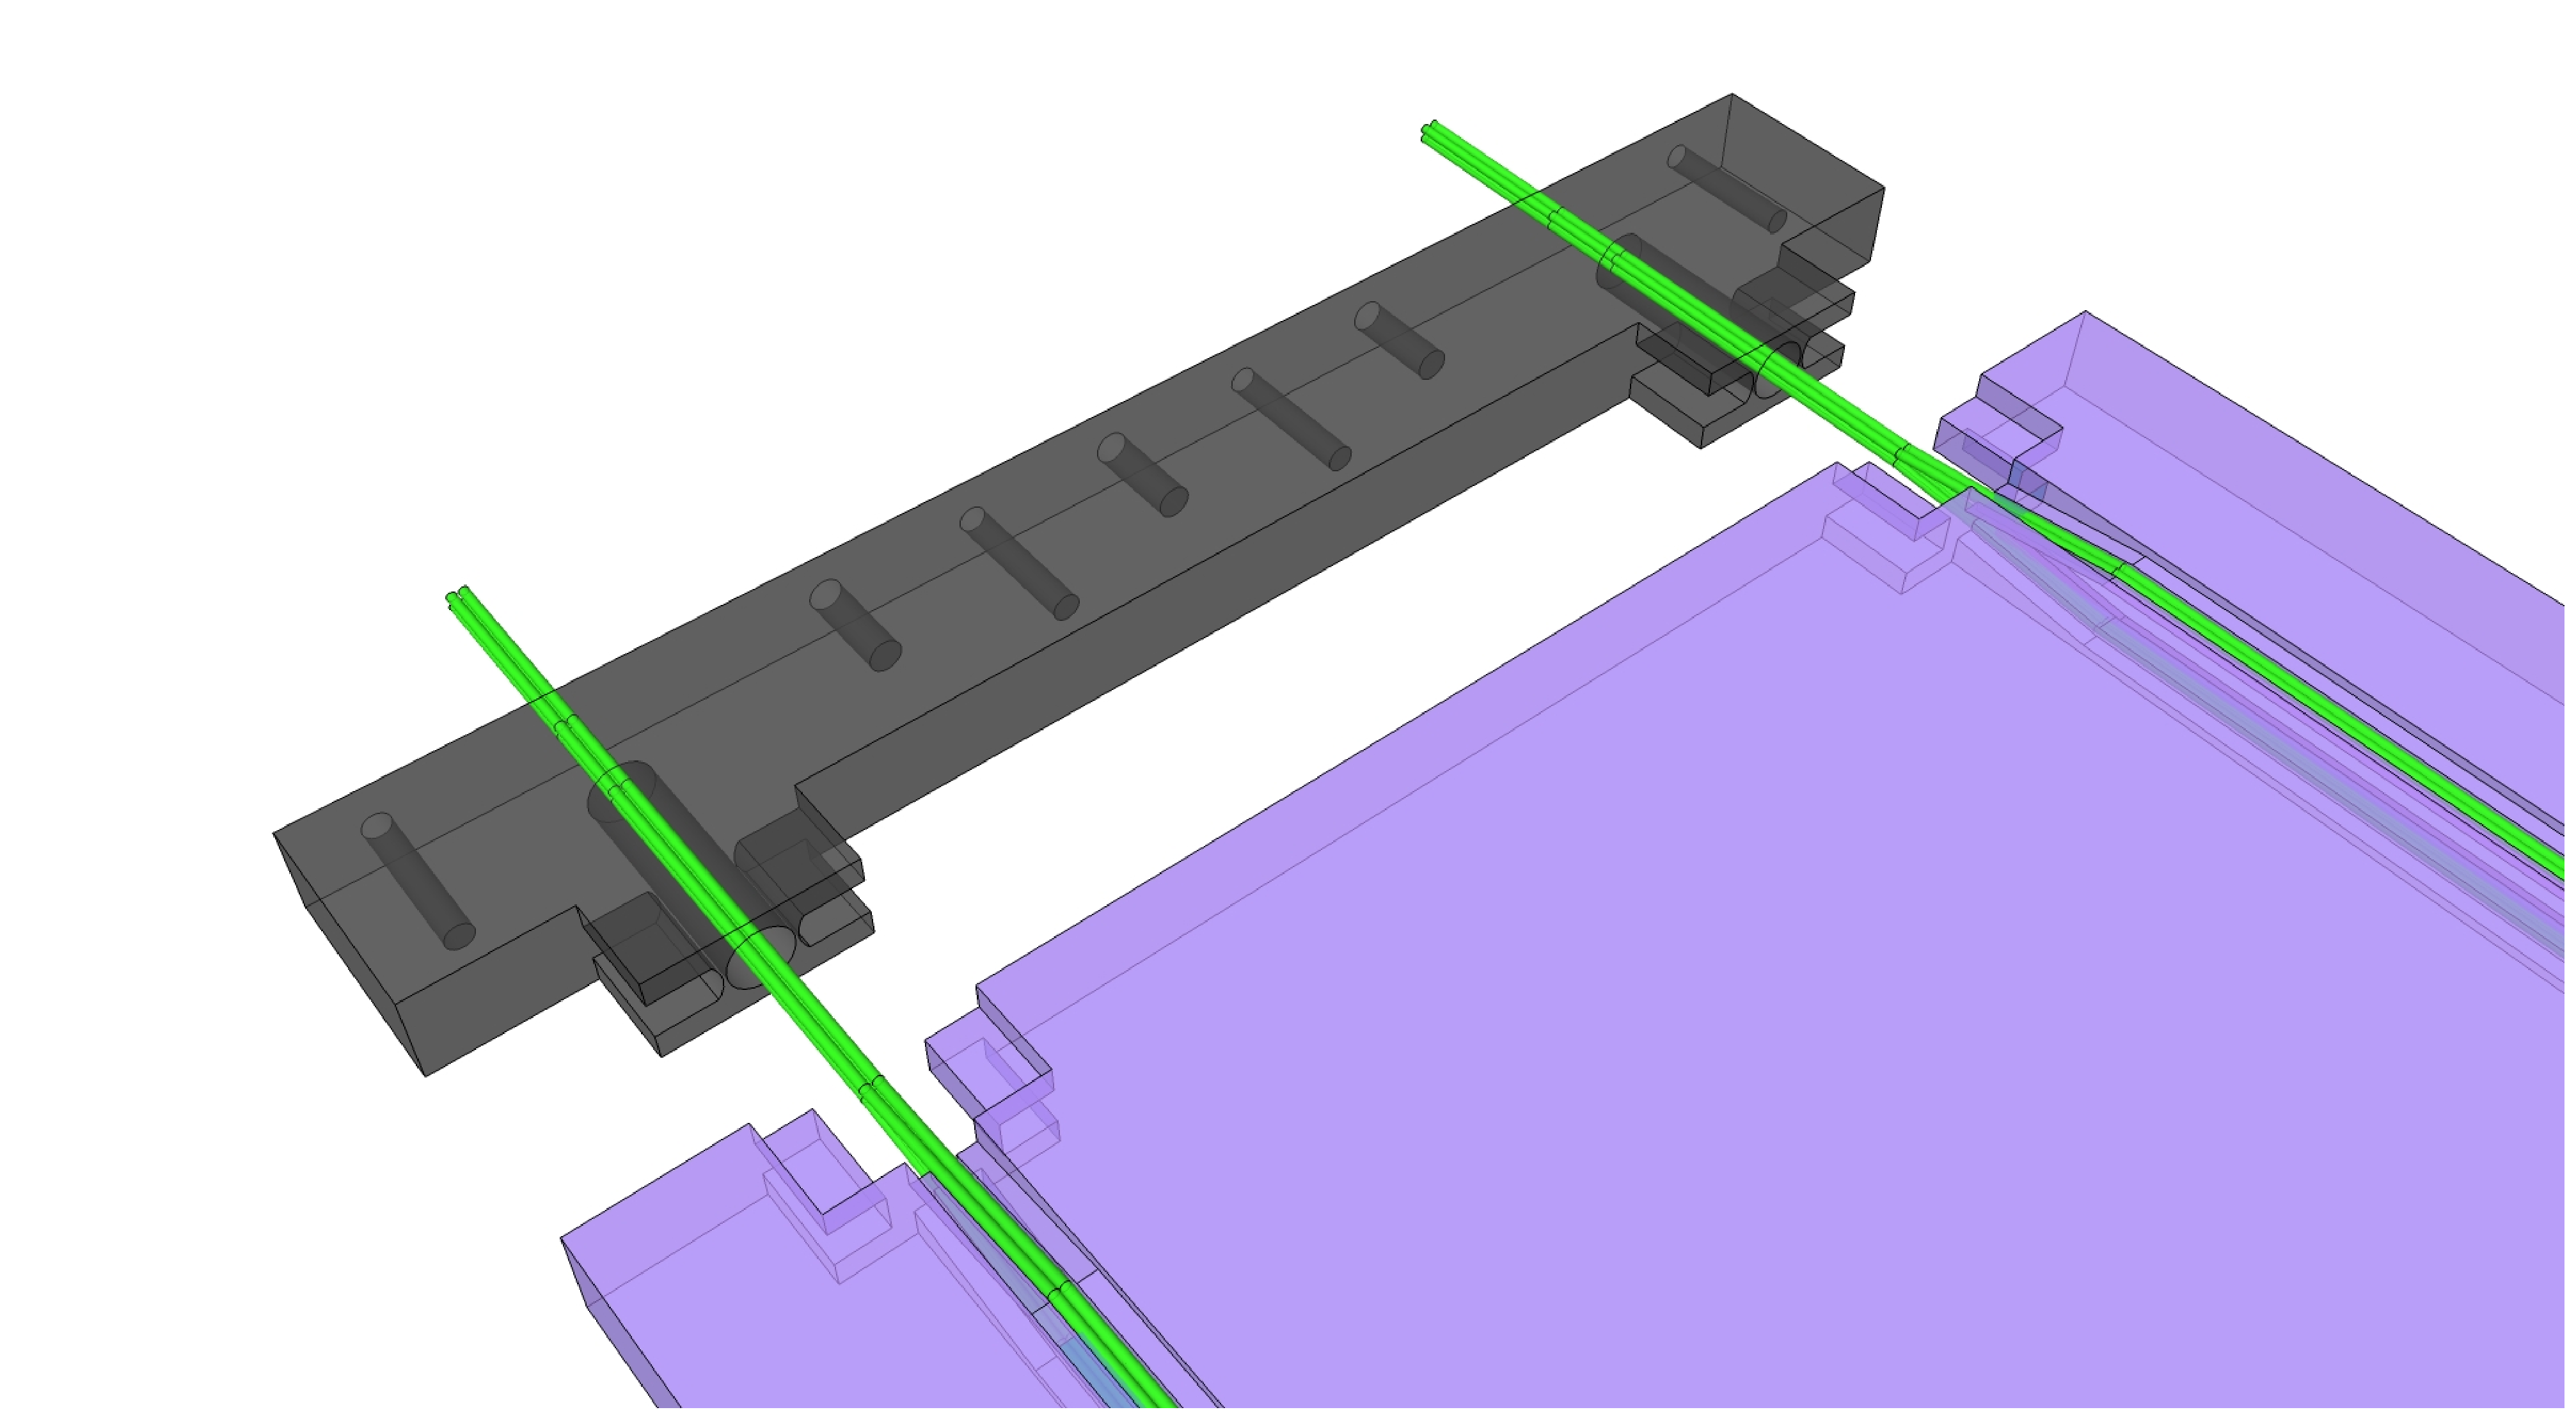
\includegraphics[width=1.0\textwidth]{figures/veto_assembly.eps}
\label{fig:paddleAssembly}
\caption{The endcap will be glued to the scintillator once it is slid into place.}
\end{figure}

\section{Paddle Performance}
\subsection{tests on intrinsic efficiency}
Show signal from detector
Talk about first tests?  Can talk about sensitivity to geometric alignment of trigger paddles ...
Maybe mention this and then be like, "this is why we decided to look at the efficiency this other way that was less sensitive"

\subsection{On-Detector Efficiency}
Initial efficiency - would be nice to show this data
Describe different cosmics that hit the neutron bar but miss the veto - argh!
Discuss changes made to mounting to improve coverage - show new data (cosmics)

\section{Electronics}
Originally wanted to use timing information but there weren't enough channels
Bit Register - give example
discuss random rate and estimate how often you'll fire druing a reall event and also how often one bar will fire with something real, vetoing a real event 

\section{Beam Tests}
What data should I show?  Old Mg vs. New Mg?  Or New Mg with no veto vs.  New Mg with veto?
show the vetoed spectrum - put a limit on how much real signal is rejected?

\subsection{Rejected Signal}
Two causes for rejected signal
1. the bars are ganged together; could get a signal in one veto bar that does not mean there was a cosmic in its adjacent neutron detector
2. randoms

can place a limit on randoms, reals, and therefore good rejected signal

% % uncomment the following lines,
% if using chapter-wise bibliography
%
% \bibliographystyle{ndnatbib}
% \bibliography{example}
